\documentclass[10.5pt]{article} 
\usepackage[utf8]{inputenc}   
\usepackage[spanish]{babel}  
\usepackage{amsmath}   
\usepackage{ amssymb }
\usepackage{amsfonts}         
\usepackage{geometry}          
\usepackage{graphicx}
\usepackage{float}
\usepackage{xcolor}
\usepackage{ulem}
\usepackage{tcolorbox}
\usepackage{cancel} 
\usepackage{tikz}
\usepackage{framed}
\usepackage{mdframed}
\usepackage{cite}
\usepackage{hyperref}

% ========================================
% CONFIGURACIÓN DE ESPACIADO AUTOMÁTICO
% ========================================
\usepackage{parskip} % Elimina sangría y añade espacio entre párrafos automáticamente

% Configuración adicional de espaciado
\setlength{\parskip}{8pt plus 2pt minus 1pt} % Espacio flexible entre párrafos
\setlength{\parindent}{0pt} % Sin sangría (no más \noindent necesario)

% Para que los espacios en blanco en el código se respeten
\usepackage{xparse}

\geometry{a4paper, margin=1in} 

\title{\textbf{Proyectos IV. Programación gráfica, sistemas inmersivos y videojuegos. Bloque 2.}}
\author{César Vidal Fernández}
\date{12 de noviembre de 2026}

\definecolor{ejercicio}{RGB}{59, 88, 102}
\definecolor{explicacion}{rgb}{0.008, 0.161, 0.098}

\newcommand{\tachareq}[1]{\textcolor{black}{\cancel{#1}}} % Para ecuaciones
\newcommand{\dvt}[1]{\;\mathrm{d}#1}
\newcommand{\separation}{\vspace{10px} \rule{\textwidth}{0.6pt} \par}
\newcommand{\lagrangian}{\mathcal{L}}
\newcommand{\ejercicio}[1]{\color{ejercicio}\textbf{\uline{#1}}\color{black}}
\newcommand{\explicacion}[1]{\color{explicacion}\textit{#1}\color{black}}

\newenvironment{sideline}
{\begin{mdframed}[
		linewidth=1pt,
		topline=false,
		bottomline=false,
		rightline=false,
		leftline=true,
		leftmargin=0cm,
		rightmargin=0cm,
		innertopmargin=0.5cm,
		innerbottommargin=0.5cm
		]}
	{\end{mdframed}}

\begin{document}
	
	\renewcommand{\contentsname}{Contenido.}
	
	\maketitle	
	\newpage
	
	\tableofcontents
	\newpage
	
	\section{Introducción y acotamiento del proyecto.}
	
	Como se expuso en el bloque anterior, la simulación constará de la representación audiovisual de un avión rompiendo la barrera del sonido en un entorno inmersivo, interactivo y ejecutado en tiempo real.
	
	Esto permite que las ecuaciones complejas de la mecánica de fluidos (tales como las ecuaciones de Navier-Stokes compresibles) sean reducidas significativamente, aplicando casos concretos o realizando simplificaciones que se detallan en la sección a continuación. 
	
	El objetivo fundamental del modelo reside en la recreación en tiempo real de la cinemática de los frentes de onda y la acústica de fuentes en movimiento con aceleración uniforme.
	
	Se estudia concretamente la aeronave \textit{Concorde}, un avión de pasajeros comercializado entre 1976 y 2003 y financiado conjuntamente por los gobiernos británico y francés. 
	
	\begin{figure}[H]
		\centering
		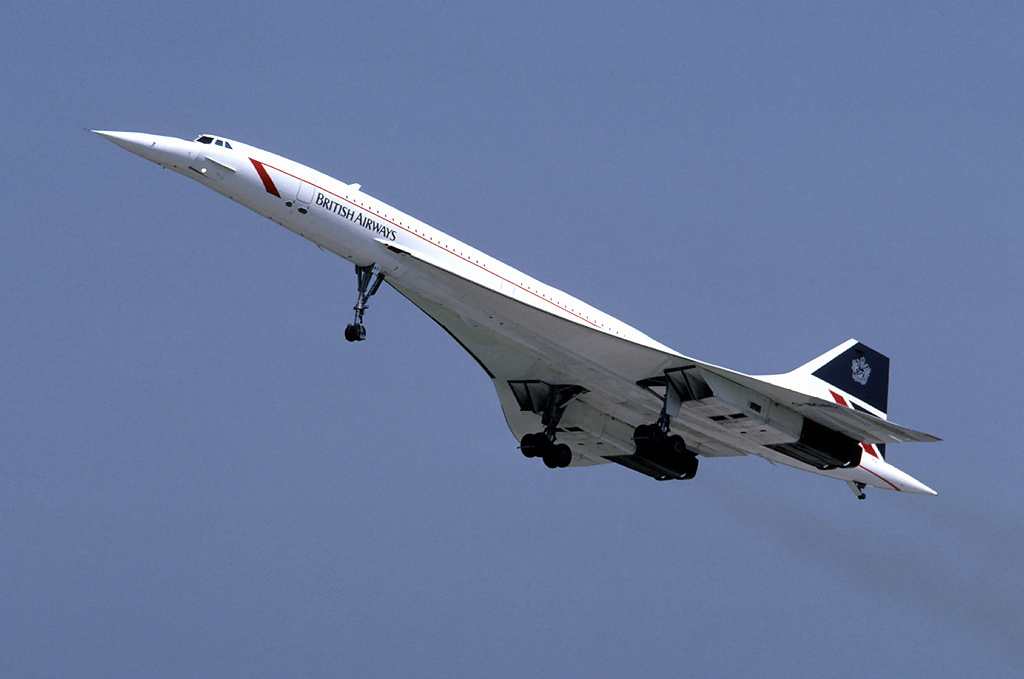
\includegraphics[width=0.6\textwidth]{imgs/concorde.jpg}
		\caption{Un Concorde de la aerolínea British Airways. Fuente: \cite{concorde_wiki}}
	\end{figure}
	
	\subsection{Terminología empleada.}
	
	\begin{itemize}
		\item Mach: unidad de velocidad en relación con la velocidad del sonido en el medio en el que se desplaza el móvil. Al nivel del mar, 1 Mach = 343 m/s. Esto es puramente una referencia; a nivel de estudio se calcula como variable dependiente de la altura. 
		
		\item Wave (onda): en el contexto de la síntesis de audio, la onda es el objeto básico y puede adoptar distintas formas según cómo queramos que responda a lo largo del tiempo. En este documento se tratarán sobre todo la onda N, que se explica de forma sencilla más adelante, y el ruido aleatorio, cuya forma de onda es, por definición, aleatoria. 
		
		\begin{figure}[H]
			\centering
			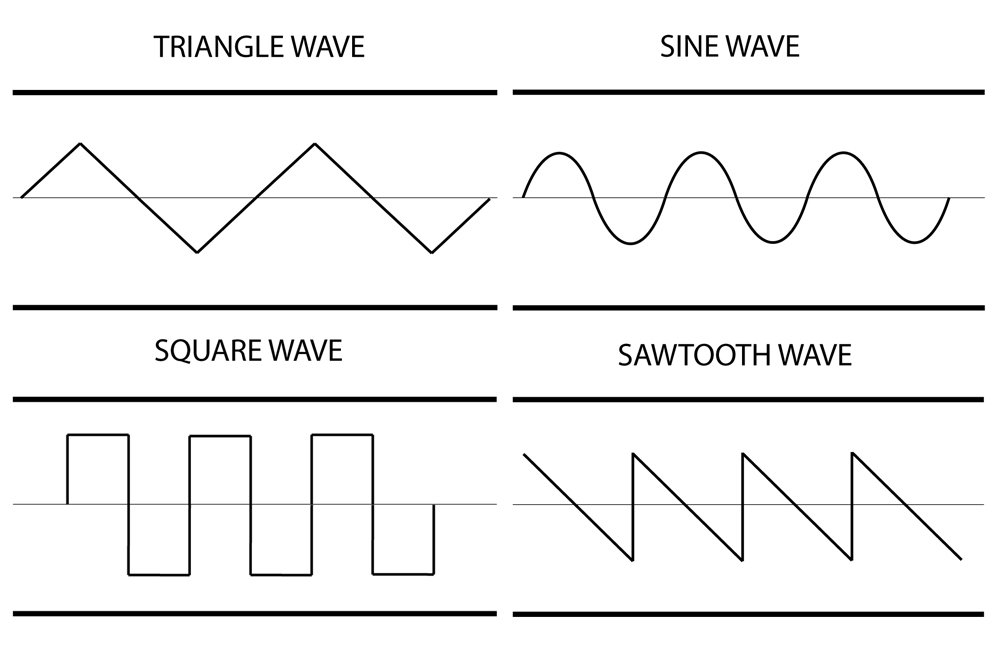
\includegraphics[width=0.5\textwidth]{imgs/waveforms.jpg}
			\caption{Formas de onda senoidal, cuadrada, triangular y de diente de sierra. Fuente: \cite{wave_forms}}
		\end{figure}
	\end{itemize}
	
	\newpage 
	\section{Ecuaciones gobernantes.}
	
	Se identifican tres bloques conceptuales y matemáticos bien diferenciados que gobiernan el comportamiento del sistema en tiempo real.
	
	\subsection{Movimiento del avión (cinemática 1D y número de Mach).}
	
	El fenómeno de interés ocurre a una velocidad elevada. Para el modelo de avión seleccionado, el \textit{Concorde}, la aceleración hacia el régimen supersónico se iniciaba a gran altitud. Se detallan a continuación las fases del vuelo para comprender de forma completa el funcionamiento de la aeronave \cite{912161}.
	
	\begin{enumerate}
		\item Fase subsónica inicial: el avión despega de forma convencional y, debido a la normativa sobre contaminación acústica cerca de las zonas pobladas, se mantiene en régimen subsónico hasta alcanzar entre 8500 y 9100 metros de altura, a una velocidad de Mach 0.95. 
		
		\item \textbf{Aceleración y ruptura de la barrera del sonido}: se encienden los motores de postcombustión, se reduce el ángulo de ataque vertical con el objetivo de comenzar un ascenso más moderado y se aumenta de forma progresiva la velocidad hasta alcanzar Mach 2 a 15200 metros.
		
		\item Crucero: el crucero se realiza a la altura y velocidad finales alcanzadas en la fase anterior. 
	\end{enumerate}
	
	Para simplificar el estudio y trabajar en una única dimensión (análogo a un problema de plano inclinado), se toman las siguientes consideraciones y simplificaciones:
	
	\begin{itemize}
		\item Se define un sistema de coordenadas rotado donde la trayectoria de ascenso del avión se realiza a lo largo de un eje inclinado un ángulo $\theta$ respecto a la horizontal.
		
		\item Se interpreta la aceleración como constante y la trayectoria de ascenso como completamente lineal.
	\end{itemize}
	
	El movimiento de la aeronave se modela considerando una distancia recorrida a lo largo de la rampa de ascenso $s(t)$, la cual experimenta un movimiento rectilíneo uniformemente acelerado:
	
	\begin{equation*}
		s(t) = s_0 + v_0 \cdot t + \frac{1}{2} \cdot a \cdot t^2
	\end{equation*}
	
	Llevando esto al plano bidimensional $(x, y)$ mediante las componentes geométricas del plano inclinado, el vector de posición de la aeronave en función del tiempo resulta:
	
	\begin{equation*}
		\vec{r}_{\text{avión}}(t) = \left( x_0 + s(t)\cos\theta, \, y_0 + s(t)\sin\theta \right)
	\end{equation*}
	
	Estableciendo el origen de tiempos $t_0 = 0$ al inicio de la fase de aceleración con velocidad inicial $v_0$ a lo largo de la rampa, el vector velocidad instantánea de la fuente en 2D es:
	
	\begin{equation*}
		\vec{v}_{\text{avión}}(t) = (a \cdot t + v_0)\cos\theta \, \hat{i} + (a \cdot t + v_0)\sin\theta \, \hat{j}
	\end{equation*}
	
	Cuya magnitud escalar a lo largo de la dirección de ascenso es:
	
	\begin{equation*}
		v_{\text{avión}}(t) = \|\vec{v}_{\text{avión}}(t)\| = a \cdot t + v_0
	\end{equation*}
	
	La velocidad del sonido ($c$) en un gas ideal depende de la temperatura local del medio ($T$):
	
	\begin{equation*}
		c(T) = \sqrt{\gamma \cdot R \cdot T}
	\end{equation*}
	
	donde $\gamma = 1.4$ es el coeficiente adiabático del aire y $R = 287\text{ J/(kg}\cdot\text{K)}$ es la constante específica del aire. Evaluando la temperatura según el modelo atmosférico de referencia a la altitud correspondiente de la rampa, se define el régimen de vuelo mediante el \textbf{número de Mach instantáneo}:
	
	\begin{equation*}
		M(t) = \frac{v_{\text{avión}}(t)}{c(T)}
	\end{equation*}
	
	\subsection{Modelo visual: propagación de frentes de onda y cáusticas.}
	
	En lugar de resolver el campo cinemático de presiones del aire, la representación visual en tiempo real se basa en el principio de Huygens. La superficie del avión actúa como un emisor continuo de esferas de perturbación sonora emitidas en cada instante $t_e$.
	
	El centro corresponde a la posición que ocupaba la aeronave en el momento de emisión. La superposición de estas esferas da lugar al cono de Mach. 
	
	\begin{figure}[H]
		\centering
		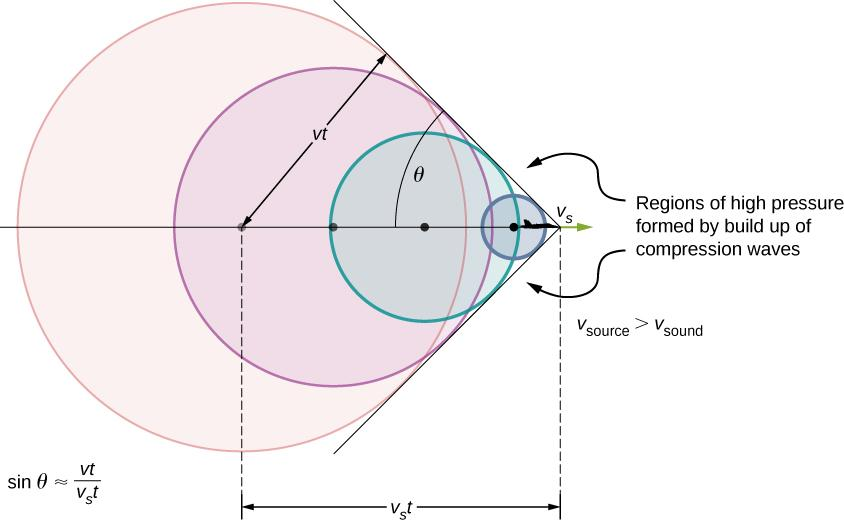
\includegraphics[width=0.6\textwidth]{imgs/rotura.jpg}
		\caption{Cono de Mach. Fuente: \cite{shockwaves}}
	\end{figure}
	
	El radio $R$ del frente de onda emitido en el instante $t_e$ y evaluado en el tiempo actual $t$ viene determinado por:
	
	\begin{equation*}
		R(t, t_e) = c \cdot (t - t_e) \qquad \text{para } t \ge t_e
	\end{equation*}
	
	La posición del centro de dicho frente es $x_{\text{emisión}} = x_{\text{avión}}(t_e)$. La acumulación o superposición de estos frentes esféricos genera la envolvente visual de la onda de choque. Cuando $M(t) > 1$, el ángulo del cono de Mach instantáneo $\mu(t)$ satisface:
	
	\begin{equation*}
		\sin(\mu(t)) = \frac{1}{M(t)}
	\end{equation*}
	
	Dado que la fuente acelera ($a > 0$), la envolvente de los frentes de onda adquiere una curvatura característica (cáustica), marcando la frontera de discontinuidad de presión visible en la atmósfera.
	
	A niveles prácticos, habrá un nivel de opacidad asociado a las esferas de Mach, en relación con su radio, para dar prioridad visual a las recién generadas.
	
	\subsection{Modelo acústico: tiempo retardado y efecto Doppler dinámico.}
	
	Para un observador situado en la posición $\mathbf{r}_{\text{obs}}$, el sonido percibido en el instante $t$ proviene de la posición que ocupaba la aeronave en el instante de emisión retardado $t_e$. Dicho instante es la solución de la ecuación del tiempo retardado:
	
	\begin{equation*}
		t - t_e = \frac{\|\mathbf{r}_{\text{obs}} - \mathbf{r}_{\text{avión}}(t_e)\|}{c}
	\end{equation*}
	
	El cambio de frecuencia percibido por el observador debido al efecto Doppler relativo con fuente en aceleración se rige por:
	
	\begin{equation*}
		f_{\text{obs}}(t) = \frac{f_0}{1 - \dfrac{\mathbf{v}_{\text{avión}}(t_e) \cdot \mathbf{n}(t_e)}{c}}
	\end{equation*}
	
	donde $\mathbf{n}(t_e) = \frac{\mathbf{r}_{\text{obs}} - \mathbf{r}_{\text{avión}}(t_e)}{\|\mathbf{r}_{\text{obs}} - \mathbf{r}_{\text{avión}}(t_e)\|}$ representa el vector unitario de la línea de visión desde la posición de emisión hacia el observador.
	
	En el momento exacto en que la envolvente de la onda de choque atraviesa la posición del observador ($\mathbf{v}_{\text{avión}} \cdot \mathbf{n} = c$), el denominador se anula teóricamente, dando lugar a la llegada simultánea de múltiples frentes de onda acumulados y generando la firma acústica de sobrepresión conocida como el \textit{boom sónico} o firma de onda en N.
	
	Pese a que el instante en que el fenómeno llega al espectador depende por completo del sistema de referencia, la intensidad percibida no lo hace, ya que existe una atenuación real directamente relacionada con el tiempo y la distancia recorridos por las ondas sonoras.
	
	\begin{equation*}
		\text{Ganancia} = \frac{1}{\|\mathbf{r}_{\text{obs}} - \mathbf{r}_{\text{avión}}(t_e)\|}
	\end{equation*}
	
	
	\subsubsection{Generación de sonido.}
	
	Se diferencian dos fuentes de sonido principales que se deberán modelar desde cero. Se decide no utilizar archivos de audio y sintetizar los sonidos mediante algoritmos numéricos, para añadir una capa de complejidad y personalización a la sonoridad general de la simulación.
	
	\begin{itemize}
		\item \textbf{Generación de ruido base (turbina)}: capa constante mientras el avión vuela. Señal modelada en cada fotograma.
		\begin{enumerate}
			\item \uline{Generación del sonido base}: se parte de un flujo de ruido blanco, es decir, aleatorio. Este sonido se filtrará mediante ecualizadores y filtros de banda para aportarle el carácter requerido. 
			
			\textit{El ruido blanco de por sí, tal y como lo conocemos, es el característico de la estática de la televisión. Necesitamos poder moldear parámetros concretos de forma precisa para convertirlo en el rugido característico de una turbina de avión.}
			
			A efectos prácticos, nos debemos centrar en las frecuencias de resonancia de los gases de escape de la turbina. Estas se encuentran típicamente alrededor de los 200, 800 y 2500 Hz. Se puede multiplicar este ruido por una señal de baja frecuencia ligeramente aleatoria, que le aportará un toque orgánico. Estos parámetros se delimitarán en fases más avanzadas del proyecto y requerirán de algo de experimentación.
			
			\item \uline{Aplicación del efecto Doppler} según el tiempo de retardo: teniendo en cuenta la posición del observador con respecto a la nave, se debe tener en cuenta el retraso debido a la limitación de la velocidad del sonido. Como resultado observable, al acercarse la nave habrá una subida en el tono, que caerá de golpe tras el cruce. 
			
			
		\end{enumerate}
		
		\item \textbf{El boom sónico}: evento aislado, que comienza en el momento en el que la onda de choque alcanza al observador. 
		
		\begin{enumerate}
			\item Construcción matemática de la onda (onda en N): como se ha contemplado en apartados anteriores, la onda expansiva tiene dos tiempos muy concretos: el instante de choque con el morro y el de choque con la parte trasera.
			
			Debido a esto se elige un pulso con forma de N, es decir, con dos momentos de sonoridad máxima, al principio y al final, y con un gran resalte alrededor de los 30--60 Hz. Con esto se pretende añadir mucho subgrave, con un \textit{decay} muy pronunciado.
			
			\item Crujido atmosférico: tras el estampido, se producen microvibraciones y un ruido de muy alta frecuencia que sucede de forma brusca.
			
			\item Reverberación: este sonido no se desvanece de forma instantánea; debido a su gran potencia sonora, es reflejado por el suelo y las capas de la atmósfera, generando un eco similar al que ocurre en una cueva o en habitaciones muy amplias. Se modelará de forma convolutiva y se establecerá una longitud temporal adecuada, que se estima entre 2 y 3 segundos. 
			
		\end{enumerate}
	\end{itemize}
	
	\newpage
	
	\section{Condiciones iniciales y de contorno.}
	
	La simulación comienza al final de la fase de ascenso inicial del Concorde, en el momento previo a iniciar la aceleración hacia el régimen supersónico. Se establece como referencia una altitud inicial de 8500 metros y una velocidad correspondiente a Mach 0.95, de acuerdo con las características operativas descritas anteriormente.
	
	A partir de este estado inicial, la aeronave comienza una fase de aceleración uniforme siguiendo una trayectoria ascendente. Se definen a continuación las condiciones iniciales del sistema, así como las restricciones geométricas y físicas que delimitan el comportamiento de la simulación.
	
	\subsection{Condiciones iniciales.}
	
	El estado inicial de la aeronave queda determinado por su posición, velocidad y aceleración. Para el instante inicial $t_0=0$, se establecen las siguientes condiciones:
	
	\begin{itemize}
		
		\item \textbf{Posición y altitud inicial:} se establece una altitud inicial de $h_0=8500$ metros. La posición horizontal inicial $x_0$ se utiliza para situar la aeronave dentro del sistema de coordenadas de la simulación.
		
		\item \textbf{Velocidad inicial:} se corresponde con el régimen de vuelo alcanzado al finalizar la fase de ascenso inicial. Se establece un número de Mach inicial de $M_0=0.95$, a partir del cual se calcula la velocidad:
		\begin{equation*}
			v_0 = M_0 \cdot c(T_0)
		\end{equation*}
		
		\item \textbf{Temperatura atmosférica:} se determina a partir de la temperatura de referencia del aire a la altitud inicial de 8500 metros. Este valor permite calcular la velocidad local del sonido mediante la expresión definida anteriormente:
		\begin{equation*}
			c(T_0) = \sqrt{\gamma R T_0}
		\end{equation*}
		
		\item \textbf{Aceleración:} se considera constante durante el intervalo de simulación. Se establece por defecto un valor de referencia correspondiente a la fase de aceleración del Concorde, aunque este parámetro podrá modificarse para estudiar diferentes comportamientos cinemáticos.
		
		\item \textbf{Inclinación de la trayectoria:} se define mediante el ángulo $\theta$ respecto a la horizontal. Su valor predeterminado reproduce la pendiente de ascenso característica de la fase de vuelo estudiada, permitiendo igualmente su modificación como parámetro de simulación.
		
		\item \textbf{Posición del observador:} se define mediante un vector de posición $\mathbf{r}_{obs}$, asociado a la posición de la cámara. Se contemplan dos configuraciones: una cámara vinculada a la aeronave, que permite observar el fenómeno desde una posición elevada respecto a ella, y una cámara de posición libre, cuyo movimiento puede controlarse independientemente de la trayectoria del avión.
		
		Aunque la cinemática de la aeronave se restringe a un plano vertical de ascenso (2D), el sistema se formula y resuelve en un entorno tridimensional (3D). Esto permite situar al observador en cualquier posición del espacio.
		
	\end{itemize}
	
	De este modo, la simulación permite estudiar la transición desde el régimen subsónico al supersónico, así como modificar determinados parámetros físicos y geométricos para observar su influencia sobre la formación de la onda de choque.
	
	\subsection{Condiciones de contorno.}
	
	Dado que el proyecto no pretende resolver directamente las ecuaciones de Navier-Stokes compresibles, sino representar la propagación geométrica de perturbaciones acústicas, no se imponen condiciones de contorno hidrodinámicas convencionales. En su lugar, se establecen las siguientes restricciones para delimitar el comportamiento del modelo:
	
	\begin{itemize}
		
		\item \textbf{Trayectoria de la aeronave:} el movimiento queda restringido a una trayectoria rectilínea definida por el ángulo de ascenso $\theta$. Durante el intervalo de simulación se mantiene constante la dirección del movimiento y se considera una aceleración uniforme.
		
		\item \textbf{Medio de propagación:} se considera el aire como un medio homogéneo e isótropo, en reposo respecto al sistema de referencia. Las perturbaciones acústicas se propagan radialmente a partir de su punto de emisión, con una velocidad determinada por las condiciones atmosféricas locales.
		
		\item \textbf{Propagación de los frentes de onda:} cada perturbación emitida por la aeronave se propaga desde la posición que ocupaba la fuente en el instante de emisión. En el modelo bidimensional, los frentes de onda se representan mediante circunferencias cuyo radio aumenta con el tiempo transcurrido desde su emisión.
		
		\item \textbf{Posición del observador:} no se establece una posición espacial fija para el observador. Su ubicación depende de la configuración de cámara seleccionada, pudiendo permanecer vinculada a la aeronave o desplazarse libremente dentro del entorno de simulación. Esta posición determina el cálculo del tiempo de recepción y del efecto Doppler.
		
		\item \textbf{Dominio espacial:} la representación visual queda limitada al área visible de la escena y al campo de visión de la cámara. Los frentes de onda que abandonan el dominio de representación dejan de visualizarse, aunque su propagación física no se considera interrumpida.
		
		\item \textbf{Dominio temporal:} la simulación se desarrolla durante un intervalo finito, actualizando continuamente el estado cinemático de la aeronave, la propagación de los frentes de onda y las señales acústicas correspondientes.
		
	\end{itemize}
	
	Estas condiciones permiten establecer un escenario controlado para estudiar la formación y propagación de la envolvente de ondas de choque, así como su percepción visual y acústica desde diferentes posiciones del entorno inmersivo.
	
	\newpage 
	
	\section{Método numérico y discretización.}
	
	\subsection{Discretización temporal.}
	
	La simulación consiste en una ejecución en tiempo real. Aunque el movimiento a estudiar es naturalmente continuo, computacionalmente debe analizarse de forma discreta.
	
	Se establece un paso temporal de cálculo de $\frac{1}{120}$ s y uno de renderizado de $\frac{1}{60}$ s, lo que equivale a 60 fps. Esto significa que por cada dos pasos de simulación se ejecuta uno de dibujado. 
	
	En fases más avanzadas del proyecto se valorará la implementación de un sistema de \textit{double buffering}, así como la modificación de estos parámetros a partir de métricas de rendimiento. 
	
	\subsection{Cálculo de la trayectoria.}
	
	Dado que se dispone de la solución analítica del movimiento, se decide evaluarla directamente en lugar de recurrir a métodos de integración numérica como el de Euler:
	\begin{equation*}
		s(t) = s_0 + v_0 \cdot t + \frac{1}{2} \cdot a \cdot t^2
	\end{equation*} 
	
	A partir de ella se pueden obtener las componentes de posición y velocidad.
	
	\subsection{Discretización de las fuentes de onda.}
	
	La emisión de perturbaciones por parte de la aeronave se lleva a cabo de forma continua, pero nuestra representación no puede ser infinita.
	Requerimos un mínimo de 10 frentes de onda por paso temporal. Esto equivale a $\Delta t_e = \frac{\Delta t}{10} = \frac{1}{120 \cdot 10} = \frac{1}{1200}$ s, es decir, 1200 Hz. Cada frente se calcula en una posición obtenida por subdivisión del intervalo entre la posición actual y la siguiente.
	
	Para cada una de estas posiciones, se debe calcular el radio en el momento simulado:
	\begin{equation*}
		R_k (t) = c(t - t_{e, k})
	\end{equation*}
	
	Los frentes fuera del área de renderizado se eliminan. 
	
	\subsection{Resolución del tiempo retardado.}
	
	Debemos resolver:
	
	\begin{equation*}
		t - t_e = \frac{\|\mathbf{r}_{\text{obs}}(t) - \mathbf{r}_{\text{avión}}(t_e)\|}{c}
	\end{equation*}
	
	Para este caso, la sustitución de valores no es posible, ya que tenemos incógnitas a ambos lados de la ecuación. Recurriremos a un método numérico de búsqueda de raíces (bisección, Newton-Raphson). El rendimiento de ambos se evaluará en fases más avanzadas del proyecto, tomando entonces la decisión de cuál elegir. 
	
	Se debe prestar especial atención a la semilla a usar para resolver el problema. En régimen supersónico pueden existir varias soluciones de tiempo para un mismo instante de recepción.
	
	\subsection{Discretización y generación de audio.}
	
	Para calcular el audio, se establece una escala completamente diferente a la de la simulación gráfica y de cálculo; para una representación fluida y con sensación de continuidad se necesita una mayor cantidad de muestras por segundo. Como referencia estándar, usaremos una frecuencia de muestreo de 44\,100 Hz:
	\begin{equation*}
		\Delta t_s = \frac{1}{44100} \approx 22.68\ \mu\text{s}
	\end{equation*}
	
	Utilizando un tamaño de bloque de 256 muestras, tendremos que procesar información cada:
	\begin{equation*}
		T_b = \frac{256}{44100} \approx 5.80\ \text{ms} \Rightarrow \text{172 bloques por segundo.}
	\end{equation*}
	
	\subsubsection{Generación del ruido blanco.}
	
	El ruido blanco se puede generar mediante una distribución gaussiana:
	\begin{equation*}
		x[n] \sim \mathcal{N}(0, \sigma ^2)
	\end{equation*}
	
	Se debe prestar especial atención a la saturación. Como punto extra, se podría intentar llevar un control de estados en el generador, para que la señal no sufra un reinicio completo en cada bloque de procesamiento.
	
	\subsubsection{Aplicación de filtros.}
	
	Sobre la señal obtenida anteriormente, podemos aplicar filtros digitales. Pretendemos modificar algunos parámetros del tono para poder modelarlo a voluntad. Como hemos mencionado anteriormente:
	
	\begin{itemize}
		\item Bandas de frecuencia y ecualizaciones para cambiar el carácter del sonido.
		\item Modulaciones de amplitud para evitar que el sonido se mantenga estático.
	\end{itemize}
	
	\begin{equation*}
		y[n] = H \cdot { x[n]} \qquad \rightarrow \text{H = sistema de filtrado}
	\end{equation*}
	
	\subsubsection{Modificación de la frecuencia mediante Doppler.}
	
	El ruido blanco, a diferencia de otros sonidos como el de un instrumento musical, no presenta una frecuencia fundamental\footnote{La frecuencia fundamental es la frecuencia más baja con la que vibra una onda periódica.}. Esto significa que no podemos simplemente modificar su parámetro de frecuencia para obtener el efecto deseado. 
	
	Ante este problema se pueden plantear diferentes soluciones. En la práctica se han de valorar las dos, pero la segunda tiene un fundamento físico más interesante y es la que, a poder ser, se debería acabar aplicando:
	
	\begin{enumerate}
		\item Generar un sonido nuevo para cada velocidad del avión. Tiene un gran problema: se debe crear una gran cantidad de sonidos para que la sensación de acercamiento y alejamiento de la aeronave tenga la continuidad y el realismo suficientes.
		
		\item Trabajar con la velocidad de reproducción del audio. No se puede cambiar una frecuencia en concreto debido a las limitaciones comentadas anteriormente, pero sí que podemos cambiar el espectro general de frecuencias mediante aceleraciones y deceleraciones de la reproducción.
		
		\begin{equation*}
			f_{\text{salida}} = k \cdot f_{\text{original}}
		\end{equation*}
		
		La selección del factor $k$ no es arbitraria, podemos obtenerla a partir de la velocidad relativa entre el Concorde y el espectador:
		% TODO: revisar esta fórmula. Aparece t_e multiplicando a v_s y cos(alpha); lo habitual sería k = c / (c - v_s cos(alpha)).
		\begin{equation*}
			k(t) = \frac{c}{c - v_s \cdot t_e \cdot \cos \alpha}
		\end{equation*}
		
		Esta solución, tal cual está establecida, presenta el mismo problema que la anterior: los saltos entre bloques. Se propone hacer una interpolación lineal entre los bloques. 
		
		\textit{Para ejemplificar esto, si la aeronave se aleja de nosotros a gran velocidad, se puede dar el caso de obtener dos factores $k$ muy diferentes para dos bloques consecutivos ($k_0 = 1.0$, $k_1 = 1.1$). Esto produciría saltos en cómo lo percibimos en la simulación, restando una gran cantidad del realismo y rigor que se pretende tener.}
		
		\begin{align*}
			k_i &= k_{\text{anterior}} + \lambda_i \left(k_{\text{nuevo}} - k_{\text{anterior}}\right) \\
			&\Rightarrow \text{$\lambda_i$ varía progresivamente entre 0 y 1.} \\
			&\Rightarrow i = \text{una muestra específica dentro de un bloque de audio.}
		\end{align*}
	\end{enumerate}
	
	\subsubsection{Generación del pulso del boom sónico.}
	
	El modelado de esta onda es ligeramente más sencillo que el de la anterior. La diferencia principal es que se puede tratar como un evento que no se ejecuta de forma constante durante el transcurso de la simulación. La única diferencia perceptible es el tratamiento de los parámetros temporales, para representar de forma adecuada el tiempo desde que sucede (desde la perspectiva del avión) hasta que lo escucha el espectador.
	
	A los demás efectos, la frecuencia de muestreo, el tamaño de bloque y otros parámetros estándar de tratamiento de audio se mantienen exactamente iguales.
	
	\subsubsection{Panorámica y espacialización del audio.}
	
	Ambos fenómenos auditivos se someterán a una capa extra de panoramización espacial en función de la posición relativa del espectador con respecto al avión, que generará una sensación de distancia junto con el control de ganancia establecido en apartados anteriores. 
	
	\section{Algoritmo y estrategia de verificación.}
	
	Esta implementación presenta tres frecuencias de actualización completamente diferentes para cinemática, renderizado y muestreo de audio. Esto supondrá gran parte de la labor, debido a la dificultad de mantener esta sincronización de forma correcta, ordenada y mantenible.  
	
	\begin{figure}[H]
		\centering
		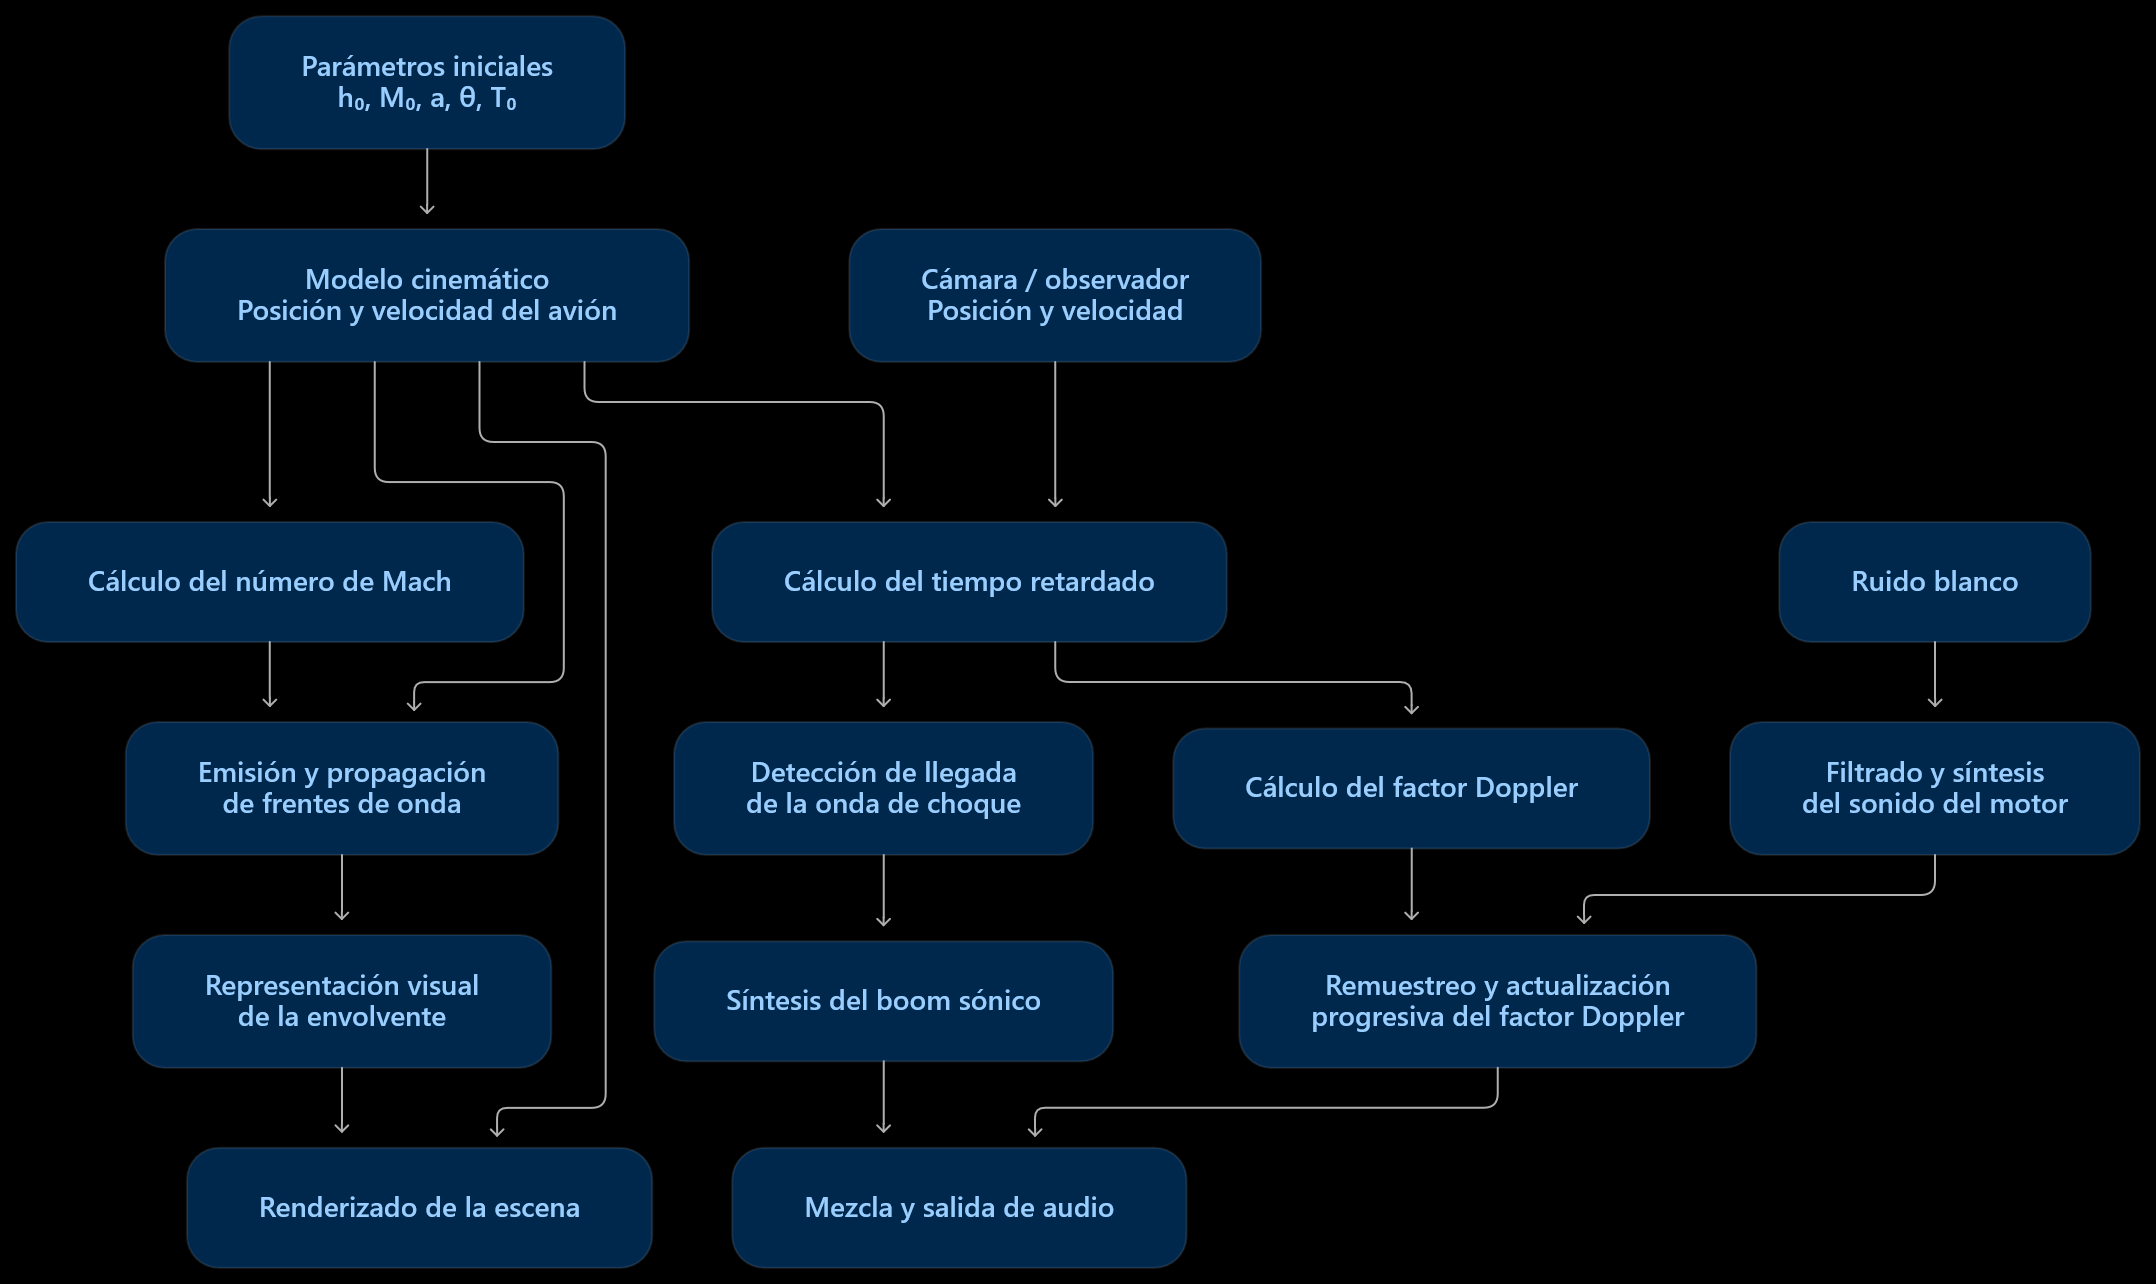
\includegraphics[width=\textwidth]{imgs/diagram.png}
	\end{figure} 
	
	\subsection{Algoritmos y métodos computacionales.}
	
	\begin{table}[H]
		\centering
		\label{tab:algoritmos}
		\begin{tabular}{|l|p{4cm}|p{10cm}|}
			\hline
			\textbf{Área} & \textbf{Algoritmo o método} & \textbf{Aplicación en el proyecto} \\
			\hline
			Cinemática &
			Evaluación analítica &
			Cálculo de la posición, velocidad y aceleración de la aeronave a partir de las ecuaciones del movimiento. \\
			\hline
			Atmósfera &
			Modelo atmosférico &
			Determinación de la temperatura y velocidad local del sonido en función de la altitud. \\
			\hline
			Ondas &
			Principio de Huygens &
			Generación de frentes de onda esféricos a partir de las posiciones anteriores de la aeronave. \\
			\hline
			Ondas &
			Cálculo de la envolvente &
			Representación de la envolvente de los frentes de onda y determinación de la geometría del cono de Mach. \\
			\hline
			Acústica &
			Resolución del tiempo retardado &
			Resolución numérica de la ecuación de propagación para determinar el instante de emisión de una señal recibida por el observador. \\
			\hline
			Acústica &
			Efecto Doppler &
			Cálculo de la variación de frecuencia percibida a partir del movimiento relativo entre la aeronave y el observador. \\
			\hline
			DSP &
			Síntesis de ruido &
			Generación de señales de ruido blanco y filtrado espectral para construir el sonido de los motores. \\
			\hline
			DSP &
			Remuestreo variable &
			Modificación de la frecuencia de reproducción de la señal para implementar el desplazamiento Doppler. \\
			\hline
			DSP &
			Síntesis del estampido sónico &
			Generación de una señal de presión tipo N asociada a la llegada de la onda de choque al observador. \\
			\hline
			Gráficos &
			Renderizado mediante shaders &
			Representación de la aeronave, geometría de los frentes de onda y efectos visuales mediante OpenGL. \\
			\hline
			Tiempo real &
			Bucle de simulación discreto &
			Actualización independiente de la física, el renderizado y el procesamiento de audio. \\
			\hline
		\end{tabular}
	\end{table}
	
	\subsection{Dependencias y librerías.}
	
	\begin{table}[H]
		\centering
		\label{tab:dependencias}
		\begin{tabular}{|l|l|p{10cm}|}
			\hline
			\textbf{Biblioteca} & \textbf{Módulo} & \textbf{Función dentro del proyecto} \\ 
			\hline
			NumPy & \texttt{numpy} &
			Operaciones vectoriales y matriciales, gestión de arrays y cálculos numéricos. \\
			\hline
			SciPy & \texttt{scipy.signal} &
			Diseño y aplicación de filtros digitales, procesamiento de señales y operaciones de interpolación. \\
			\hline
			SciPy & \texttt{scipy.optimize} &
			Resolución numérica de ecuaciones no lineales, especialmente para el cálculo del tiempo retardado. \\
			\hline
			ModernGL & \texttt{moderngl} &
			Renderizado gráfico mediante OpenGL, gestión de shaders y representación de geometrías y frentes de onda. \\
			\hline
			SoundDevice & \texttt{sounddevice} &
			Reproducción y generación de audio en tiempo real mediante dispositivos de salida. \\
			\hline
			SoundFile & \texttt{soundfile} &
			Lectura y escritura de archivos de audio, principalmente en formato WAV. \\
			\hline
			Matplotlib & \texttt{matplotlib} &
			Representación gráfica de resultados, análisis de señales y validación de los modelos. \\
			\hline
			Librosa & \texttt{librosa} &
			Análisis de señales de audio, representación tiempo-frecuencia y extracción de características espectrales. \\
			\hline
			Pytest & \texttt{pytest} &
			Automatización de pruebas unitarias para comprobar el funcionamiento de los distintos módulos. \\
			\hline
		\end{tabular}
	\end{table}
	
	\subsection{Pruebas y validación del sistema.}
	
	\begin{table}[H]
		\centering
		\label{tab:tests}
		\begin{tabular}{|l|p{4cm}|p{10cm}|}
			\hline
			\textbf{Área} & \textbf{Prueba} & \textbf{Criterio de validación} \\
			\hline
			Cinemática &
			Validación de la trayectoria &
			Comparación de la posición y velocidad calculadas con las soluciones analíticas del modelo de movimiento. \\
			\hline
			Atmósfera &
			Validación de la velocidad del sonido &
			Comprobación de la coherencia de la temperatura y velocidad del sonido obtenidas para distintas altitudes. \\
			\hline
			Ondas &
			Validación del ángulo de Mach &
			Comparación de la geometría de la envolvente de los frentes de onda con la relación teórica $\sin(\mu)=1/M$. \\
			\hline
			Acústica &
			Validación del tiempo retardado &
			Comprobación del residuo de la ecuación de propagación y de la coherencia temporal de las soluciones obtenidas. \\
			\hline
			Acústica &
			Validación del efecto Doppler &
			Comparación de la frecuencia sintetizada con la frecuencia teórica para distintos movimientos relativos entre fuente y observador. \\
			\hline
			DSP &
			Validación del remuestreo &
			Comprobación del desplazamiento de frecuencia mediante señales de prueba de frecuencia conocida. \\
			\hline
			DSP &
			Continuidad entre bloques de audio &
			Detección de discontinuidades en las muestras generadas en las transiciones entre bloques consecutivos. \\
			\hline
			DSP &
			Validación del estampido sónico &
			Comprobación de la generación del evento acústico cuando el frente de choque alcanza la posición del observador. \\
			\hline
			Gráficos &
			Validación del renderizado &
			Comprobación de la correspondencia entre la geometría calculada por el modelo físico y su representación gráfica. \\
			\hline
			Sistema &
			Rendimiento en tiempo real &
			Medición de la tasa de fotogramas, carga de CPU y estabilidad de la reproducción de audio. \\
			\hline
			Sistema &
			Convergencia numérica &
			Comparación de los resultados al reducir el paso temporal y el intervalo entre emisiones de frentes de onda. \\
			\hline
		\end{tabular}
	\end{table}
	
	\subsection{Estructura del proyecto.}
	
	\begin{table}[H]
		\centering
		\label{tab:estructura}
		\begin{tabular}{|l|p{4cm}|p{10cm}|}
			\hline
			\textbf{Directorio} & \textbf{Módulo} & \textbf{Responsabilidad} \\
			\hline
			\texttt{physics/} &
			\texttt{trajectory.py} &
			Cálculo de la posición, velocidad y aceleración de la aeronave. \\
			\cline{2-3}
			&
			\texttt{atmosphere.py} &
			Modelo atmosférico y cálculo de la velocidad local del sonido. \\
			\cline{2-3}
			&
			\texttt{wavefronts.py} &
			Generación y actualización de los frentes de onda. \\
			\hline
			\texttt{acoustics/} &
			\texttt{retarded\_time.py} &
			Resolución del tiempo de emisión correspondiente a cada instante de recepción. \\
			\cline{2-3}
			&
			\texttt{doppler.py} &
			Cálculo del desplazamiento de frecuencia debido al movimiento relativo. \\
			\cline{2-3}
			&
			\texttt{sonic\_boom.py} &
			Detección de la llegada de la onda de choque y generación del evento acústico. \\
			\hline
			\texttt{dsp/} &
			\texttt{noise.py} &
			Generación de las señales de ruido utilizadas para la síntesis sonora. \\
			\cline{2-3}
			&
			\texttt{filters.py} &
			Diseño y aplicación de filtros digitales. \\
			\cline{2-3}
			&
			\texttt{resampling.py} &
			Remuestreo de señales con una relación de frecuencia variable. \\
			\cline{2-3}
			&
			\texttt{audio\_engine.py} &
			Gestión del flujo de audio y reproducción en tiempo real. \\
			\hline
			\texttt{visualization/} &
			\texttt{renderer.py} &
			Gestión del contexto OpenGL y renderizado mediante ModernGL. \\
			\cline{2-3}
			&
			\texttt{shaders/} &
			Programas GLSL para el procesamiento gráfico de vértices y fragmentos. \\
			\cline{2-3}
			&
			\texttt{camera.py} &
			Gestión de la cámara y de las transformaciones espaciales. \\
			\hline
			\texttt{analysis/} &
			\texttt{spectral\_analysis.py} &
			Análisis espectral y representación de las señales generadas. \\
			\cline{2-3}
			&
			\texttt{convergence.py} &
			Evaluación de la convergencia numérica del modelo. \\
			\cline{2-3}
			&
			\texttt{benchmarks.py} &
			Medición del rendimiento computacional. \\
			\hline
			\texttt{tests/} &
			\texttt{test\_*.py} &
			Pruebas unitarias y de integración de los distintos módulos. \\
			\hline
			Directorio raíz &
			\texttt{main.py} &
			Inicialización y coordinación de los subsistemas de simulación. \\
			\cline{2-3}
			&
			\texttt{requirements.txt} &
			Declaración de las dependencias externas del proyecto. \\
			\hline
		\end{tabular}
		
	\end{table}
	
	\newpage
	\begin{verbatim}
		concorde_simulation/
		|
		|-- main.py
		|-- requirements.txt
		|
		|-- physics/
		|   |-- trajectory.py
		|   |-- atmosphere.py
		|   |-- wavefronts.py
		|
		|-- acoustics/
		|   |-- retarded_time.py
		|   |-- doppler.py
		|   |-- sonic_boom.py
		|
		|-- dsp/
		|   |-- noise.py
		|   |-- filters.py
		|   |-- resampling.py
		|   |-- audio_engine.py
		|
		|-- visualization/
		|   |-- renderer.py
		|   |-- camera.py
		|   |-- shaders/
		|
		|-- analysis/
		|   |-- spectral_analysis.py
		|   |-- convergence.py
		|   |-- benchmarks.py
		|
		|-- tests/
		|   |-- test_trajectory.py
		|   |-- test_doppler.py
		|   |-- test_wavefronts.py
		|   |-- test_audio.py
	\end{verbatim}
	
	\newpage 
	
	\section{Planificación de tareas hasta febrero.}
	
	El desarrollo del proyecto se distribuirá en distintas etapas comprendidas entre noviembre de 2026 y febrero de 2027. La planificación establece una implementación progresiva de los diferentes subsistemas, comenzando por el modelo físico y continuando con los módulos acústicos, el procesamiento digital de señales y la representación gráfica. Finalmente, se realizará la integración de los componentes, la validación de los resultados y la elaboración de la documentación técnica.
	
	Las tareas se organizarán de manera modular, permitiendo desarrollar y verificar cada subsistema de forma independiente antes de su integración en la aplicación principal.
	
	\begin{table}[H]
		\centering
		\label{tab:planificacion}
		\small
		\begin{tabular}{|c|p{3.1cm}|c|p{2.5cm}|p{2.5cm}|p{2.5cm}|}
			\hline
			\textbf{ID} & \textbf{Tarea} & \textbf{Duración} &
			\textbf{Responsable} & \textbf{Dependencias} &
			\textbf{Hito} \\
			\hline
			T1 & Preparación del entorno y arquitectura del proyecto &
			1 semana & Desarrollo principal & Ninguna &
			Estructura inicial operativa \\
			\hline
			T2 & Implementación y validación del modelo cinemático y atmosférico &
			2 semanas & Desarrollo principal & T1 &
			Modelo físico funcional \\
			\hline
			T3 & Generación de frentes de onda y envolvente de Mach &
			2 semanas & Desarrollo principal & T2 &
			Modelo geométrico validado \\
			\hline
			T4 & Implementación del tiempo retardado y propagación acústica &
			3 semanas & Desarrollo principal & T2, T3 &
			Modelo de propagación operativo \\
			\hline
			T5 & Implementación del efecto Doppler y síntesis del estampido sónico &
			2 semanas & Desarrollo principal & T4 &
			Modelo acústico completo \\
			\hline
			T6 & Desarrollo del motor de audio y procesamiento DSP &
			3 semanas & Desarrollo principal & T5 &
			Audio generado en tiempo real \\
			\hline
			T7 & Desarrollo del renderizador mediante ModernGL y shaders &
			3 semanas & Desarrollo principal & T3 &
			Representación gráfica funcional \\
			\hline
			T8 & Integración de los subsistemas físico, gráfico y acústico &
			2 semanas & Desarrollo principal & T5, T6, T7 &
			Primera versión integrada \\
			\hline
			T9 & Pruebas, validación numérica y optimización &
			2 semanas & Desarrollo principal & T8 &
			Versión estable validada \\
			\hline
			T10 & Documentación, resultados y memoria final &
			2 semanas & Desarrollo principal & T9 &
			Entrega final \\
			\hline
		\end{tabular}
	\end{table}
	
	\newpage
	
	\section{Referencias.}
	
	\bibliographystyle{plain} 
	\bibliography{references}
	
\end{document}